\section{Section 1.3 - Basic Functions}  	
  	\subsection{Question 1}
  		What we see here is that:
  
  		\begin{itemize}
 
  		\item The further the non-zero point $(p,q)$ from the origin $O(0,0)$, the smaller the wavelength of the spatial image 
  		(more dense lines in the real and imaginary part of the spatial image),
  
  		\item The amplitude of all the spatial images is the same,
  
  		\item The direction of the waveforms in the spatial images is dictated by the position of the non-zero point $(p,q)$ relative to the origin $O(0,0)$
  
  		\end{itemize}
  		
  		
  		The output of the \texttt{fftwave} function for $(p,q)=(5,9)$, $(p,q)=(9,5)$, $(p,q)=(17,9)$, $(p,q)=(17,121)$, $(p,q)=(5,1)$ and $(p,q)=(125,1)$
  		is illustrated in figures \ref{fig:59}, \ref{fig:95}, \ref{fig:179}, \ref{fig:17121}, \ref{fig:51} and \ref{fig:1251} respectively.

	  	\begin{figure}[H]
			\centering
			\scalebox{0.7}{% This file was created by matlab2tikz.
%
%The latest updates can be retrieved from
%  http://www.mathworks.com/matlabcentral/fileexchange/22022-matlab2tikz-matlab2tikz
%where you can also make suggestions and rate matlab2tikz.
%
\begin{tikzpicture}

\begin{axis}[%
width=1.484in,
height=1.484in,
at={(3.399in,4.935in)},
scale only axis,
axis on top,
xmin=0.5,
xmax=128.5,
y dir=reverse,
ymin=0.5,
ymax=128.5,
hide axis,
title style={font=\bfseries},
title={Fhat: (u, v) = (5, 9)}
]
\addplot [forget plot] graphics [xmin=0.5,xmax=128.5,ymin=0.5,ymax=128.5] {./images/Q1/a1.png};
\end{axis}

\begin{axis}[%
width=1.484in,
height=1.484in,
at={(6.532in,4.935in)},
scale only axis,
axis on top,
xmin=0.5,
xmax=128.5,
y dir=reverse,
ymin=0.5,
ymax=128.5,
hide axis,
title style={font=\bfseries},
title={centered Fhat: (uc, vc) = (4, 8)}
]
\addplot [forget plot] graphics [xmin=0.5,xmax=128.5,ymin=0.5,ymax=128.5] {./images/Q1/a2.png};
\end{axis}

\begin{axis}[%
width=1.484in,
height=1.484in,
at={(3.399in,2.85in)},
scale only axis,
axis on top,
xmin=0.5,
xmax=128.5,
y dir=reverse,
ymin=0.5,
ymax=128.5,
hide axis,
title style={font=\bfseries},
title={real(F)}
]
\addplot [forget plot] graphics [xmin=0.5,xmax=128.5,ymin=0.5,ymax=128.5] {./images/Q1/a3.png};
\end{axis}

\begin{axis}[%
width=1.484in,
height=1.484in,
at={(6.532in,2.85in)},
scale only axis,
axis on top,
xmin=0.5,
xmax=128.5,
y dir=reverse,
ymin=0.5,
ymax=128.5,
hide axis,
title style={font=\bfseries},
title={imag(F)}
]
\addplot [forget plot] graphics [xmin=0.5,xmax=128.5,ymin=0.5,ymax=128.5] {./images/Q1/a4.png};
\end{axis}

\begin{axis}[%
width=1.484in,
height=1.484in,
at={(3.399in,0.765in)},
scale only axis,
axis on top,
xmin=0.5,
xmax=128.5,
y dir=reverse,
ymin=0.5,
ymax=128.5,
hide axis,
title style={font=\bfseries},
title={abs(F) (amplitude 0.000061)}
]
\addplot [forget plot] graphics [xmin=0.5,xmax=128.5,ymin=0.5,ymax=128.5] {./images/Q1/a5.png};
\end{axis}

\begin{axis}[%
width=1.484in,
height=1.484in,
at={(6.532in,0.765in)},
scale only axis,
axis on top,
xmin=0.5,
xmax=128.5,
y dir=reverse,
ymin=0.5,
ymax=128.5,
hide axis,
title style={font=\bfseries},
title={angle(F) (wavelength 14.310835)}
]
\addplot [forget plot] graphics [xmin=0.5,xmax=128.5,ymin=0.5,ymax=128.5] {./images/Q1/a6.png};
\end{axis}
\end{tikzpicture}%}
			\caption{$(p,q)=(5,9)$}
			\label{fig:59}
	  	\end{figure}
	  	
	  	\begin{figure}[H]
			\centering
			\scalebox{0.7}{% This file was created by matlab2tikz.
%
%The latest updates can be retrieved from
%  http://www.mathworks.com/matlabcentral/fileexchange/22022-matlab2tikz-matlab2tikz
%where you can also make suggestions and rate matlab2tikz.
%
\begin{tikzpicture}

\begin{axis}[%
width=1.484in,
height=1.484in,
at={(3.399in,4.935in)},
scale only axis,
axis on top,
xmin=0.5,
xmax=128.5,
y dir=reverse,
ymin=0.5,
ymax=128.5,
hide axis,
title style={font=\bfseries},
title={Fhat: (u, v) = (9, 5)}
]
\addplot [forget plot] graphics [xmin=0.5,xmax=128.5,ymin=0.5,ymax=128.5] {./images/Q1/b1.png};
\end{axis}

\begin{axis}[%
width=1.484in,
height=1.484in,
at={(6.532in,4.935in)},
scale only axis,
axis on top,
xmin=0.5,
xmax=128.5,
y dir=reverse,
ymin=0.5,
ymax=128.5,
hide axis,
title style={font=\bfseries},
title={centered Fhat: (uc, vc) = (8, 4)}
]
\addplot [forget plot] graphics [xmin=0.5,xmax=128.5,ymin=0.5,ymax=128.5] {./images/Q1/b2.png};
\end{axis}

\begin{axis}[%
width=1.484in,
height=1.484in,
at={(3.399in,2.85in)},
scale only axis,
axis on top,
xmin=0.5,
xmax=128.5,
y dir=reverse,
ymin=0.5,
ymax=128.5,
hide axis,
title style={font=\bfseries},
title={real(F)}
]
\addplot [forget plot] graphics [xmin=0.5,xmax=128.5,ymin=0.5,ymax=128.5] {./images/Q1/b3.png};
\end{axis}

\begin{axis}[%
width=1.484in,
height=1.484in,
at={(6.532in,2.85in)},
scale only axis,
axis on top,
xmin=0.5,
xmax=128.5,
y dir=reverse,
ymin=0.5,
ymax=128.5,
hide axis,
title style={font=\bfseries},
title={imag(F)}
]
\addplot [forget plot] graphics [xmin=0.5,xmax=128.5,ymin=0.5,ymax=128.5] {./images/Q1/b4.png};
\end{axis}

\begin{axis}[%
width=1.484in,
height=1.484in,
at={(3.399in,0.765in)},
scale only axis,
axis on top,
xmin=0.5,
xmax=128.5,
y dir=reverse,
ymin=0.5,
ymax=128.5,
hide axis,
title style={font=\bfseries},
title={abs(F) (amplitude 0.000061)}
]
\addplot [forget plot] graphics [xmin=0.5,xmax=128.5,ymin=0.5,ymax=128.5] {./images/Q1/b5.png};
\end{axis}

\begin{axis}[%
width=1.484in,
height=1.484in,
at={(6.532in,0.765in)},
scale only axis,
axis on top,
xmin=0.5,
xmax=128.5,
y dir=reverse,
ymin=0.5,
ymax=128.5,
hide axis,
title style={font=\bfseries},
title={angle(F) (wavelength 14.310835)}
]
\addplot [forget plot] graphics [xmin=0.5,xmax=128.5,ymin=0.5,ymax=128.5] {./images/Q1/b6.png};
\end{axis}
\end{tikzpicture}%}
			\caption{$(p,q)=(9,5)$}
			\label{fig:95}
	  	\end{figure}

	  	\begin{figure}[H]
			\centering
			\scalebox{0.7}{% This file was created by matlab2tikz.
%
%The latest updates can be retrieved from
%  http://www.mathworks.com/matlabcentral/fileexchange/22022-matlab2tikz-matlab2tikz
%where you can also make suggestions and rate matlab2tikz.
%
\begin{tikzpicture}

\begin{axis}[%
width=1.484in,
height=1.484in,
at={(3.399in,4.935in)},
scale only axis,
axis on top,
xmin=0.5,
xmax=128.5,
y dir=reverse,
ymin=0.5,
ymax=128.5,
hide axis,
title style={font=\bfseries},
title={Fhat: (u, v) = (17, 9)}
]
\addplot [forget plot] graphics [xmin=0.5,xmax=128.5,ymin=0.5,ymax=128.5] {./images/Q1/c1.png};
\end{axis}

\begin{axis}[%
width=1.484in,
height=1.484in,
at={(6.532in,4.935in)},
scale only axis,
axis on top,
xmin=0.5,
xmax=128.5,
y dir=reverse,
ymin=0.5,
ymax=128.5,
hide axis,
title style={font=\bfseries},
title={centered Fhat: (uc, vc) = (16, 8)}
]
\addplot [forget plot] graphics [xmin=0.5,xmax=128.5,ymin=0.5,ymax=128.5] {./images/Q1/c2.png};
\end{axis}

\begin{axis}[%
width=1.484in,
height=1.484in,
at={(3.399in,2.85in)},
scale only axis,
axis on top,
xmin=0.5,
xmax=128.5,
y dir=reverse,
ymin=0.5,
ymax=128.5,
hide axis,
title style={font=\bfseries},
title={real(F)}
]
\addplot [forget plot] graphics [xmin=0.5,xmax=128.5,ymin=0.5,ymax=128.5] {./images/Q1/c3.png};
\end{axis}

\begin{axis}[%
width=1.484in,
height=1.484in,
at={(6.532in,2.85in)},
scale only axis,
axis on top,
xmin=0.5,
xmax=128.5,
y dir=reverse,
ymin=0.5,
ymax=128.5,
hide axis,
title style={font=\bfseries},
title={imag(F)}
]
\addplot [forget plot] graphics [xmin=0.5,xmax=128.5,ymin=0.5,ymax=128.5] {./images/Q1/c4.png};
\end{axis}

\begin{axis}[%
width=1.484in,
height=1.484in,
at={(3.399in,0.765in)},
scale only axis,
axis on top,
xmin=0.5,
xmax=128.5,
y dir=reverse,
ymin=0.5,
ymax=128.5,
hide axis,
title style={font=\bfseries},
title={abs(F) (amplitude 0.000061)}
]
\addplot [forget plot] graphics [xmin=0.5,xmax=128.5,ymin=0.5,ymax=128.5] {./images/Q1/c5.png};
\end{axis}

\begin{axis}[%
width=1.484in,
height=1.484in,
at={(6.532in,0.765in)},
scale only axis,
axis on top,
xmin=0.5,
xmax=128.5,
y dir=reverse,
ymin=0.5,
ymax=128.5,
hide axis,
title style={font=\bfseries},
title={angle(F) (wavelength 7.155418)}
]
\addplot [forget plot] graphics [xmin=0.5,xmax=128.5,ymin=0.5,ymax=128.5] {./images/Q1/c6.png};
\end{axis}
\end{tikzpicture}%}
			\caption{$(p,q)=(17,9)$}
			\label{fig:179}
	  	\end{figure}
	  	
	  	\begin{figure}[H]
			\centering
			\scalebox{0.7}{% This file was created by matlab2tikz.
%
%The latest updates can be retrieved from
%  http://www.mathworks.com/matlabcentral/fileexchange/22022-matlab2tikz-matlab2tikz
%where you can also make suggestions and rate matlab2tikz.
%
\begin{tikzpicture}

\begin{axis}[%
width=1.484in,
height=1.484in,
at={(3.399in,4.935in)},
scale only axis,
axis on top,
xmin=0.5,
xmax=128.5,
y dir=reverse,
ymin=0.5,
ymax=128.5,
hide axis,
title style={font=\bfseries},
title={Fhat: (u, v) = (17, 121)}
]
\addplot [forget plot] graphics [xmin=0.5,xmax=128.5,ymin=0.5,ymax=128.5] {./images/Q1/d1.png};
\end{axis}

\begin{axis}[%
width=1.484in,
height=1.484in,
at={(6.532in,4.935in)},
scale only axis,
axis on top,
xmin=0.5,
xmax=128.5,
y dir=reverse,
ymin=0.5,
ymax=128.5,
hide axis,
title style={font=\bfseries},
title={centered Fhat: (uc, vc) = (16, -8)}
]
\addplot [forget plot] graphics [xmin=0.5,xmax=128.5,ymin=0.5,ymax=128.5] {./images/Q1/d2.png};
\end{axis}

\begin{axis}[%
width=1.484in,
height=1.484in,
at={(3.399in,2.85in)},
scale only axis,
axis on top,
xmin=0.5,
xmax=128.5,
y dir=reverse,
ymin=0.5,
ymax=128.5,
hide axis,
title style={font=\bfseries},
title={real(F)}
]
\addplot [forget plot] graphics [xmin=0.5,xmax=128.5,ymin=0.5,ymax=128.5] {./images/Q1/d3.png};
\end{axis}

\begin{axis}[%
width=1.484in,
height=1.484in,
at={(6.532in,2.85in)},
scale only axis,
axis on top,
xmin=0.5,
xmax=128.5,
y dir=reverse,
ymin=0.5,
ymax=128.5,
hide axis,
title style={font=\bfseries},
title={imag(F)}
]
\addplot [forget plot] graphics [xmin=0.5,xmax=128.5,ymin=0.5,ymax=128.5] {./images/Q1/d4.png};
\end{axis}

\begin{axis}[%
width=1.484in,
height=1.484in,
at={(3.399in,0.765in)},
scale only axis,
axis on top,
xmin=0.5,
xmax=128.5,
y dir=reverse,
ymin=0.5,
ymax=128.5,
hide axis,
title style={font=\bfseries},
title={abs(F) (amplitude 0.000061)}
]
\addplot [forget plot] graphics [xmin=0.5,xmax=128.5,ymin=0.5,ymax=128.5] {./images/Q1/d5.png};
\end{axis}

\begin{axis}[%
width=1.484in,
height=1.484in,
at={(6.532in,0.765in)},
scale only axis,
axis on top,
xmin=0.5,
xmax=128.5,
y dir=reverse,
ymin=0.5,
ymax=128.5,
hide axis,
title style={font=\bfseries},
title={angle(F) (wavelength 7.155418)}
]
\addplot [forget plot] graphics [xmin=0.5,xmax=128.5,ymin=0.5,ymax=128.5] {./images/Q1/d6.png};
\end{axis}
\end{tikzpicture}%}
			\caption{$(p,q)=(17,121)$}
			\label{fig:17121}
	  	\end{figure}
	  	
	  	\begin{figure}[H]
			\centering
			\scalebox{0.7}{% This file was created by matlab2tikz.
%
%The latest updates can be retrieved from
%  http://www.mathworks.com/matlabcentral/fileexchange/22022-matlab2tikz-matlab2tikz
%where you can also make suggestions and rate matlab2tikz.
%
\begin{tikzpicture}

\begin{axis}[%
width=1.484in,
height=1.484in,
at={(3.399in,4.935in)},
scale only axis,
axis on top,
xmin=0.5,
xmax=128.5,
y dir=reverse,
ymin=0.5,
ymax=128.5,
hide axis,
title style={font=\bfseries},
title={Fhat: (u, v) = (5, 1)}
]
\addplot [forget plot] graphics [xmin=0.5,xmax=128.5,ymin=0.5,ymax=128.5] {./images/Q1/e1.png};
\end{axis}

\begin{axis}[%
width=1.484in,
height=1.484in,
at={(6.532in,4.935in)},
scale only axis,
axis on top,
xmin=0.5,
xmax=128.5,
y dir=reverse,
ymin=0.5,
ymax=128.5,
hide axis,
title style={font=\bfseries},
title={centered Fhat: (uc, vc) = (4, 0)}
]
\addplot [forget plot] graphics [xmin=0.5,xmax=128.5,ymin=0.5,ymax=128.5] {./images/Q1/e2.png};
\end{axis}

\begin{axis}[%
width=1.484in,
height=1.484in,
at={(3.399in,2.85in)},
scale only axis,
axis on top,
xmin=0.5,
xmax=128.5,
y dir=reverse,
ymin=0.5,
ymax=128.5,
hide axis,
title style={font=\bfseries},
title={real(F)}
]
\addplot [forget plot] graphics [xmin=0.5,xmax=128.5,ymin=0.5,ymax=128.5] {./images/Q1/e3.png};
\end{axis}

\begin{axis}[%
width=1.484in,
height=1.484in,
at={(6.532in,2.85in)},
scale only axis,
axis on top,
xmin=0.5,
xmax=128.5,
y dir=reverse,
ymin=0.5,
ymax=128.5,
hide axis,
title style={font=\bfseries},
title={imag(F)}
]
\addplot [forget plot] graphics [xmin=0.5,xmax=128.5,ymin=0.5,ymax=128.5] {./images/Q1/e4.png};
\end{axis}

\begin{axis}[%
width=1.484in,
height=1.484in,
at={(3.399in,0.765in)},
scale only axis,
axis on top,
xmin=0.5,
xmax=128.5,
y dir=reverse,
ymin=0.5,
ymax=128.5,
hide axis,
title style={font=\bfseries},
title={abs(F) (amplitude 0.000061)}
]
\addplot [forget plot] graphics [xmin=0.5,xmax=128.5,ymin=0.5,ymax=128.5] {./images/Q1/e5.png};
\end{axis}

\begin{axis}[%
width=1.484in,
height=1.484in,
at={(6.532in,0.765in)},
scale only axis,
axis on top,
xmin=0.5,
xmax=128.5,
y dir=reverse,
ymin=0.5,
ymax=128.5,
hide axis,
title style={font=\bfseries},
title={angle(F) (wavelength 32.000000)}
]
\addplot [forget plot] graphics [xmin=0.5,xmax=128.5,ymin=0.5,ymax=128.5] {./images/Q1/e6.png};
\end{axis}
\end{tikzpicture}%}
			\caption{$(p,q)=(5,1)$}
			\label{fig:51}
	  	\end{figure}
	  	
	  	\begin{figure}[H]
			\centering
			\scalebox{0.7}{% This file was created by matlab2tikz.
%
%The latest updates can be retrieved from
%  http://www.mathworks.com/matlabcentral/fileexchange/22022-matlab2tikz-matlab2tikz
%where you can also make suggestions and rate matlab2tikz.
%
\begin{tikzpicture}

\begin{axis}[%
width=1.484in,
height=1.484in,
at={(3.399in,4.935in)},
scale only axis,
axis on top,
xmin=0.5,
xmax=128.5,
y dir=reverse,
ymin=0.5,
ymax=128.5,
hide axis,
title style={font=\bfseries},
title={Fhat: (u, v) = (125, 1)}
]
\addplot [forget plot] graphics [xmin=0.5,xmax=128.5,ymin=0.5,ymax=128.5] {./images/Q1/f1.png};
\end{axis}

\begin{axis}[%
width=1.484in,
height=1.484in,
at={(6.532in,4.935in)},
scale only axis,
axis on top,
xmin=0.5,
xmax=128.5,
y dir=reverse,
ymin=0.5,
ymax=128.5,
hide axis,
title style={font=\bfseries},
title={centered Fhat: (uc, vc) = (-4, 0)}
]
\addplot [forget plot] graphics [xmin=0.5,xmax=128.5,ymin=0.5,ymax=128.5] {./images/Q1/f2.png};
\end{axis}

\begin{axis}[%
width=1.484in,
height=1.484in,
at={(3.399in,2.85in)},
scale only axis,
axis on top,
xmin=0.5,
xmax=128.5,
y dir=reverse,
ymin=0.5,
ymax=128.5,
hide axis,
title style={font=\bfseries},
title={real(F)}
]
\addplot [forget plot] graphics [xmin=0.5,xmax=128.5,ymin=0.5,ymax=128.5] {./images/Q1/f3.png};
\end{axis}

\begin{axis}[%
width=1.484in,
height=1.484in,
at={(6.532in,2.85in)},
scale only axis,
axis on top,
xmin=0.5,
xmax=128.5,
y dir=reverse,
ymin=0.5,
ymax=128.5,
hide axis,
title style={font=\bfseries},
title={imag(F)}
]
\addplot [forget plot] graphics [xmin=0.5,xmax=128.5,ymin=0.5,ymax=128.5] {./images/Q1/f4.png};
\end{axis}

\begin{axis}[%
width=1.484in,
height=1.484in,
at={(3.399in,0.765in)},
scale only axis,
axis on top,
xmin=0.5,
xmax=128.5,
y dir=reverse,
ymin=0.5,
ymax=128.5,
hide axis,
title style={font=\bfseries},
title={abs(F) (amplitude 0.000061)}
]
\addplot [forget plot] graphics [xmin=0.5,xmax=128.5,ymin=0.5,ymax=128.5] {./images/Q1/f5.png};
\end{axis}

\begin{axis}[%
width=1.484in,
height=1.484in,
at={(6.532in,0.765in)},
scale only axis,
axis on top,
xmin=0.5,
xmax=128.5,
y dir=reverse,
ymin=0.5,
ymax=128.5,
hide axis,
title style={font=\bfseries},
title={angle(F) (wavelength 32.000000)}
]
\addplot [forget plot] graphics [xmin=0.5,xmax=128.5,ymin=0.5,ymax=128.5] {./images/Q1/f6.png};
\end{axis}
\end{tikzpicture}%}
			\caption{$(p,q)=(125,1)$}
			\label{fig:1251}
	  	\end{figure}
	  	
	  	
  	\subsection{Question 2}
  
  		We exploit equation $4.2-33$ from \cite{GZ}  
  
  		\begin{equation}
  			\sum_{x=0}^{M-1}\sum_{y=0}^{N-1} s(x,y) \cdot A \delta(x-x_0, y-y_0) = A \cdot s(x_0, y_0)
  		\end{equation}
  
  		knowing that the output Fourier transform is a delta function at $(p,q)$. Hence, for a quadratic image $M=N$ and in the spatial domain:
  
  		\begin{equation}
  			f(x,y)= \frac{1}{N^2} \sum_{x=0}^{N-1}\sum_{y=0}^{N-1} \delta(u - p, v - q) \cdot e^{\dfrac{2 \pi i \cdot (xu + yv)}{N}} = 
  			\frac{1}{N^2} \cdot e^{\dfrac{2 \pi i \cdot (px + qy)}{N}}
  		\end{equation}
  
	  	Hence, 
	  	\begin{equation}
	  		f(x,y) = \frac{1}{N^2} \cdot (\cos(\dfrac{2 \pi \cdot (px + qy)}{N}) + i\sin(\dfrac{2 \pi \cdot (px + qy)}{N}))
	  		\label{eq:q2:sin_form}
	  	\end{equation}
	  	
	  	The spatial image for $(p,q)=(5,9)$ is plotted in figure \ref{fig:q2_1}.
	  	The real part of equation \ref{eq:q2:sin_form} is plotted in figure \ref{fig:q2_2}.
  
  	  	\begin{figure}[H]
			\centering
			\scalebox{.6}{% This file was created by matlab2tikz.
%
%The latest updates can be retrieved from
%  http://www.mathworks.com/matlabcentral/fileexchange/22022-matlab2tikz-matlab2tikz
%where you can also make suggestions and rate matlab2tikz.
%
\begin{tikzpicture}

\begin{axis}[%
width=3.566in,
height=3.566in,
at={(1.236in,0.481in)},
scale only axis,
axis on top,
xmin=0.5,
xmax=128.5,
y dir=reverse,
ymin=0.5,
ymax=128.5,
hide axis
]
\addplot [forget plot] graphics [xmin=0.5,xmax=128.5,ymin=0.5,ymax=128.5] {./images/Q2/black-1.png};
\end{axis}
\end{tikzpicture}%}
			\caption{The inverse Fourier transform of an image for $(p,q)=(5,9)$.}
			\label{fig:q2_1}
	  	\end{figure}
  
	  	\begin{figure}[H]
			\centering
			\scalebox{.6}{% This file was created by matlab2tikz.
%
%The latest updates can be retrieved from
%  http://www.mathworks.com/matlabcentral/fileexchange/22022-matlab2tikz-matlab2tikz
%where you can also make suggestions and rate matlab2tikz.
%
\definecolor{mycolor1}{rgb}{0.00000,0.44700,0.74100}%
%
\begin{tikzpicture}

\begin{axis}[%
width=4.521in,
height=3.566in,
at={(0.758in,0.481in)},
scale only axis,
xmin=0,
xmax=140,
ymin=-0.008,
ymax=0.008,
axis background/.style={fill=white}
]
\addplot [color=mycolor1,solid,forget plot]
  table[row sep=crcr]{%
1	0.00195748866460033\\
2	0.0037366152086228\\
3	0.00529177840245197\\
4	0.00652976566209381\\
5	0.00737637513408318\\
6	0.00778086316860173\\
7	0.00771898576666483\\
8	0.00719445170465574\\
9	0.00623870023956485\\
10	0.0049090167187246\\
11	0.00328509903966998\\
12	0.00146428075791393\\
13	-0.00044430284241422\\
14	-0.00232625604396381\\
15	-0.00406877928874101\\
16	-0.00556743010089505\\
17	-0.0067323831069475\\
18	-0.00749381394354109\\
19	-0.00780608435477231\\
20	-0.00765047763486313\\
21	-0.0070363204605939\\
22	-0.00600042387367352\\
23	-0.00460487691916207\\
24	-0.00293332518372927\\
25	-0.00108595728883801\\
26	0.000826500164114749\\
27	0.00268941926876141\\
28	0.00439114132316963\\
29	0.00582966937257579\\
30	0.00691878165120943\\
31	0.00759319949882841\\
32	0.0078125\\
33	0.00756353883233632\\
34	0.0068612381042336\\
35	0.00574769196109545\\
36	0.00428964356776166\\
37	0.00257448469049206\\
38	0.000705017653534714\\
39	-0.00120670637452706\\
40	-0.00304610344697526\\
41	-0.00470292471353221\\
42	-0.00607786446011923\\
43	-0.00708851224445987\\
44	-0.00767429237143736\\
45	-0.00780009464843351\\
46	-0.00745837880227468\\
47	-0.00666962642430676\\
48	-0.00548111335514479\\
49	-0.00396407608927815\\
50	-0.00220944203813713\\
51	-0.000322379568951686\\
52	0.00158400552358809\\
53	0.00339544929517815\\
54	0.00500337834633231\\
55	0.00631141743982026\\
56	0.00724116599083312\\
57	0.00773689720153487\\
58	0.00776889818565135\\
59	0.00733525088440154\\
60	0.00646194703013342\\
61	0.00520133026703267\\
62	0.00362895880428341\\
63	0.00183907664638817\\
64	-6.10351562499502e-05\\
65	-0.00195748866460029\\
66	-0.00373661520862282\\
67	-0.00529177840245198\\
68	-0.00652976566209382\\
69	-0.00737637513408317\\
70	-0.00778086316860173\\
71	-0.00771898576666483\\
72	-0.00719445170465573\\
73	-0.00623870023956483\\
74	-0.00490901671872463\\
75	-0.00328509903967001\\
76	-0.00146428075791396\\
77	0.000444302842414243\\
78	0.00232625604396383\\
79	0.00406877928874099\\
80	0.00556743010089503\\
81	0.00673238310694748\\
82	0.0074938139435411\\
83	0.00780608435477231\\
84	0.00765047763486312\\
85	0.00703632046059392\\
86	0.00600042387367354\\
87	0.0046048769191621\\
88	0.00293332518372925\\
89	0.00108595728883799\\
90	-0.000826500164114717\\
91	-0.00268941926876138\\
92	-0.0043911413231696\\
93	-0.00582966937257581\\
94	-0.00691878165120944\\
95	-0.00759319949882842\\
96	-0.0078125\\
97	-0.00756353883233634\\
98	-0.00686123810423365\\
99	-0.00574769196109544\\
100	-0.00428964356776164\\
101	-0.00257448469049204\\
102	-0.000705017653534691\\
103	0.00120670637452697\\
104	0.00304610344697529\\
105	0.00470292471353223\\
106	0.00607786446011925\\
107	0.00708851224445988\\
108	0.00767429237143734\\
109	0.00780009464843351\\
110	0.00745837880227467\\
111	0.00666962642430674\\
112	0.00548111335514477\\
113	0.00396407608927813\\
114	0.00220944203813722\\
115	0.000322379568951663\\
116	-0.00158400552358811\\
117	-0.00339544929517817\\
118	-0.00500337834633232\\
119	-0.00631141743982021\\
120	-0.00724116599083313\\
121	-0.00773689720153487\\
122	-0.00776889818565135\\
123	-0.00733525088440153\\
124	-0.00646194703013347\\
125	-0.00520133026703274\\
126	-0.00362895880428339\\
127	-0.00183907664638814\\
128	6.10351562499732e-05\\
};
\end{axis}
\end{tikzpicture}%}
			\caption{The real part of the spatial image above.}
			\label{fig:q2_2}
	  	\end{figure}


	\subsection{Question 3}

		As can be seen in equation \ref{eq:q2:sin_form}, the amplitude of the waveform is
	
		\begin{equation}
			A = \dfrac{1}{N^2}
		\end{equation}
	
	\subsection{Question 4}
	
		As seen in the lecture notes, 
		
		\begin{equation}
			\lambda = \frac{2 \pi}{|\omega|}
			\label{q4:eq:wavelength}
		\end{equation}
		
		and 
		
		\begin{equation}
			\omega = [\frac{2 \pi u}{N} \ \frac{2 \pi v}{N}]^T
		\end{equation}
		
		Hence, equation \ref{q4:eq:wavelength} for $(u,v)=(p,q)$ becomes
		
		\begin{equation}
			\lambda = \frac{1}{\sqrt{p^2+q^2}}
		\end{equation}
		
		The direction of travel of the waveforms in the spatial images is dictated by the position of the non-zero point $(p,q)$ relative to the origin $O(0,0)$.
		Figure \ref{fig:Q4} illustrates the dependence of the direction of a waveform on $p = \frac{\omega_l N}{2 \pi}$ and $q = \frac{\omega_k N}{2 \pi}$.
		
		\begin{figure}
			\centering
			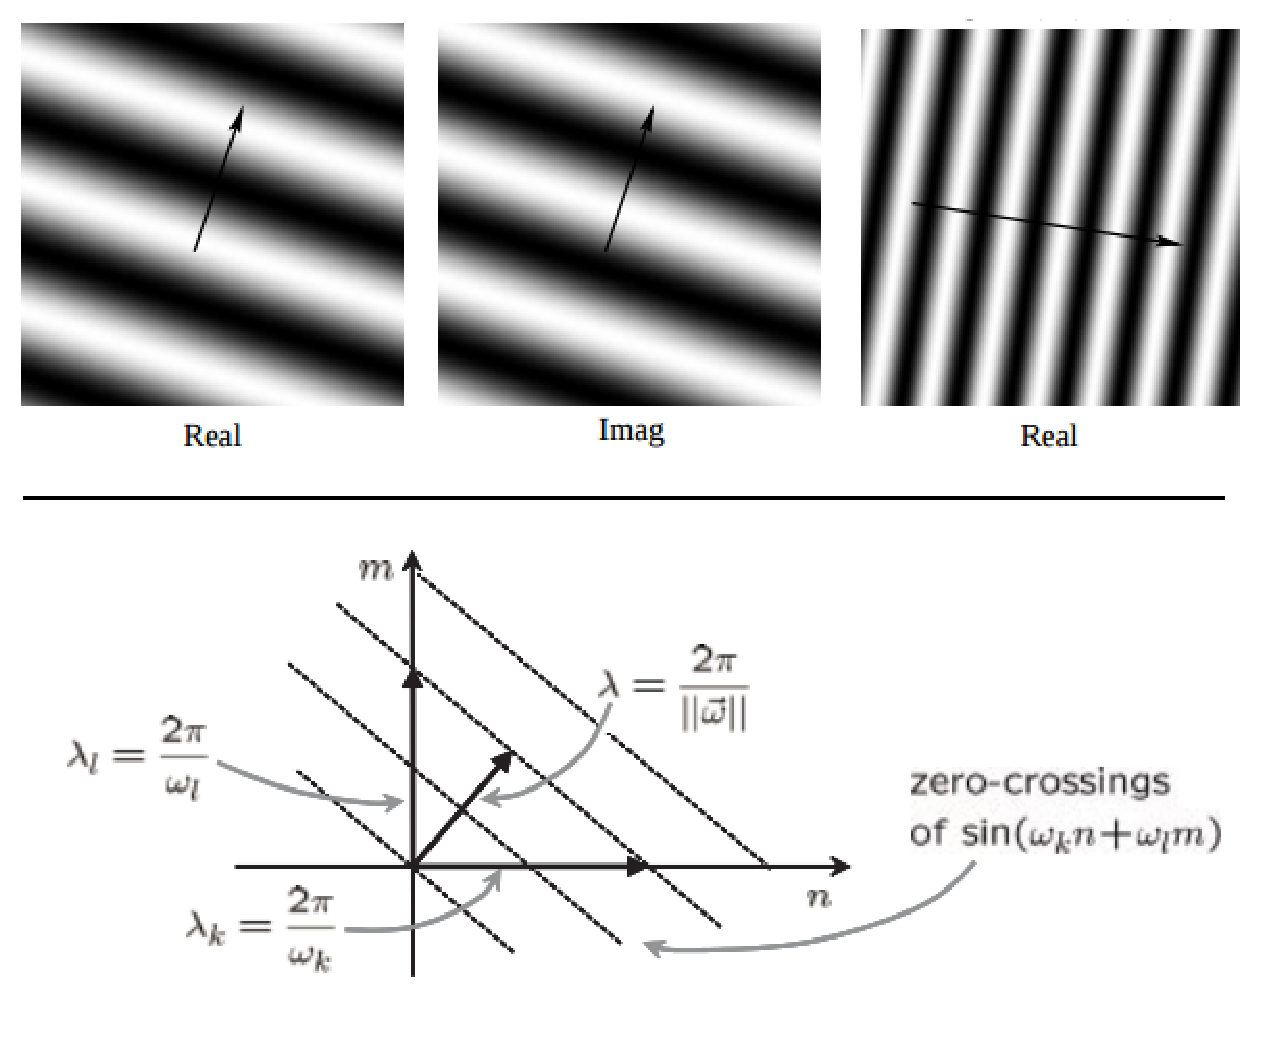
\includegraphics[scale=0.4]{./images/Q4/wavelength.eps}
			\caption{Image taken from Allan$_+$ Jepson's notes (\texttt{www.cs.toronto.edu/\~jepson/csc320/notes/linearFilters2.pdf})}
			\label{fig:Q4}		
		\end{figure}
		
		
		
	\subsection{Question 5}
	
		For an quadratic image of size $N$, the highest number of cycles that can fit in it is $N/2$, that is, stripes of width of $1$ pixel.
		The corresponding (maximum) frequency is $\omega_{max}$ = $2\pi / 2 = \pi$. However, 
		
		\begin{equation}
		\omega = \frac{2\pi u}{N} \leq \omega_{max}	
		\end{equation}				
				
		Hence, when either $p$ or $q$ exceed the value of $N/2$, which in our case is $N/2 = 64$, the Nyquist frequency is exceeded
		and the corresponding waveform in the spatial domain is no longer a sinusoid. Figure \ref{fig:q5} illustrates the waveform of the
		real part of a spatial image whose Fourier transform is an image with a non-zero pixel located at $(p,q)=(69,120)$.
		
		\begin{figure}[H]
			\centering
			\scalebox{.4}{% This file was created by matlab2tikz.
%
%The latest updates can be retrieved from
%  http://www.mathworks.com/matlabcentral/fileexchange/22022-matlab2tikz-matlab2tikz
%where you can also make suggestions and rate matlab2tikz.
%
\definecolor{mycolor1}{rgb}{0.00000,0.44700,0.74100}%
%
\begin{tikzpicture}

\begin{axis}[%
width=10.793in,
height=5.671in,
at={(1.811in,0.765in)},
scale only axis,
xmin=0,
xmax=140,
ymin=-0.002,
ymax=0.002,
axis background/.style={fill=white}
]
\addplot [color=mycolor1,solid,forget plot]
  table[row sep=crcr]{%
1	0.0011761405011441\\
2	-0.00150132552114309\\
3	0.00173652485231055\\
4	-0.00186764123623756\\
5	0.00188681588550005\\
6	-0.00179289951968045\\
7	0.00159152125035495\\
8	-0.00129475118625478\\
9	0.000920376981200602\\
10	-0.000490837686716064\\
11	3.18788115201923e-05\\
12	0.000428990799737703\\
13	-0.000864147777677171\\
14	0.00124750990371305\\
15	-0.00155609941286574\\
16	0.00177142022340174\\
17	-0.00188056654561545\\
18	0.00187699642251639\\
19	-0.00176092383833509\\
20	0.00153930589284421\\
21	-0.00122542581023588\\
22	0.000838096775955735\\
23	-0.0004005343215214\\
24	-6.10351562498684e-05\\
25	0.000518946339733578\\
26	-0.00094575318029509\\
27	0.00131587394565499\\
28	-0.00160712452480459\\
29	0.00180204808801667\\
30	-0.00188896140546677\\
31	0.00186265511074541\\
32	-0.00172470593722446\\
33	0.00148338221261035\\
34	-0.00115314827610533\\
35	0.000753797522168983\\
36	-0.000309266034063528\\
37	-0.000153802084982475\\
38	0.000607651692542704\\
39	-0.00102508018066348\\
40	0.0013810679320049\\
41	-0.00165427793299569\\
42	0.00182833466094679\\
43	-0.00189280559183885\\
44	0.00184382649966333\\
45	-0.00168433306844467\\
46	0.00142388493469737\\
47	-0.00107809270677394\\
48	0.000667682304126462\\
49	-0.000217252697641091\\
50	-0.000246198491020887\\
51	0.000694893159200493\\
52	-0.00110193767309024\\
53	0.00144293480473935\\
54	-0.00169744604074858\\
55	0.0018502166155355\\
56	-0.00189208984375\\
57	0.00182055594904343\\
58	-0.00163990249377283\\
59	0.00136095739325911\\
60	-0.00100043991768217\\
61	0.000579958580931237\\
62	-0.000124715980440949\\
63	-0.000338001783329989\\
64	0.000780460567372316\\
65	-0.00117614050114418\\
66	0.00150132552114302\\
67	-0.00173652485231059\\
68	0.00186764123623754\\
69	-0.00188681588550006\\
70	0.00179289951968042\\
71	-0.00159152125035501\\
72	0.00129475118625471\\
73	-0.000920376981200516\\
74	0.000490837686716177\\
75	-3.1878811520094e-05\\
76	-0.000428990799737589\\
77	0.000864147777677067\\
78	-0.00124750990371312\\
79	0.00155609941286568\\
80	-0.00177142022340178\\
81	0.00188056654561543\\
82	-0.0018769964225164\\
83	0.00176092383833505\\
84	-0.00153930589284428\\
85	0.0012254258102358\\
86	-0.000838096775955647\\
87	0.000400534321521514\\
88	6.10351562499666e-05\\
89	-0.000518946339733466\\
90	0.000945753180294988\\
91	-0.00131587394565506\\
92	0.00160712452480453\\
93	-0.0018020480880167\\
94	0.00188896140546678\\
95	-0.00186265511074543\\
96	0.00172470593722451\\
97	-0.00148338221261029\\
98	0.00115314827610542\\
99	-0.000753797522169091\\
100	0.000309266034063431\\
101	0.000153802084982573\\
102	-0.000607651692542594\\
103	0.00102508018066357\\
104	-0.00138106793200497\\
105	0.00165427793299564\\
106	-0.00182833466094676\\
107	0.00189280559183885\\
108	-0.00184382649966336\\
109	0.00168433306844472\\
110	-0.0014238849346973\\
111	0.00107809270677404\\
112	-0.000667682304126571\\
113	0.000217252697640994\\
114	0.000246198491020984\\
115	-0.000694893159200384\\
116	0.00110193767309032\\
117	-0.00144293480473942\\
118	0.00169744604074853\\
119	-0.00185021661553547\\
120	0.00189208984375\\
121	-0.00182055594904346\\
122	0.00163990249377289\\
123	-0.00136095739325904\\
124	0.00100043991768227\\
125	-0.000579958580931348\\
126	0.00012471598044085\\
127	0.000338001783330086\\
128	-0.000780460567372209\\
};
\end{axis}
\end{tikzpicture}%}
			\caption{Example waveform in the spatial domain for $(p,q)=(69,120)$}
			\label{fig:q5}
	  	\end{figure}
	  	
	
	\subsection{Question 6}
	
		The purpose of these lines is to visualize the mapping of the angular frequency values $\omega_x$ and $\omega_y$ inside the interval
	
		\begin{equation}
			-\pi \leq \omega_x, \omega_y \leq \pi
		\end{equation}
		
		The exact operation is performed by \texttt{fftshift()} function.